\documentclass{standalone}
\usepackage{tikz}
\usetikzlibrary{patterns, positioning}


\begin{document}
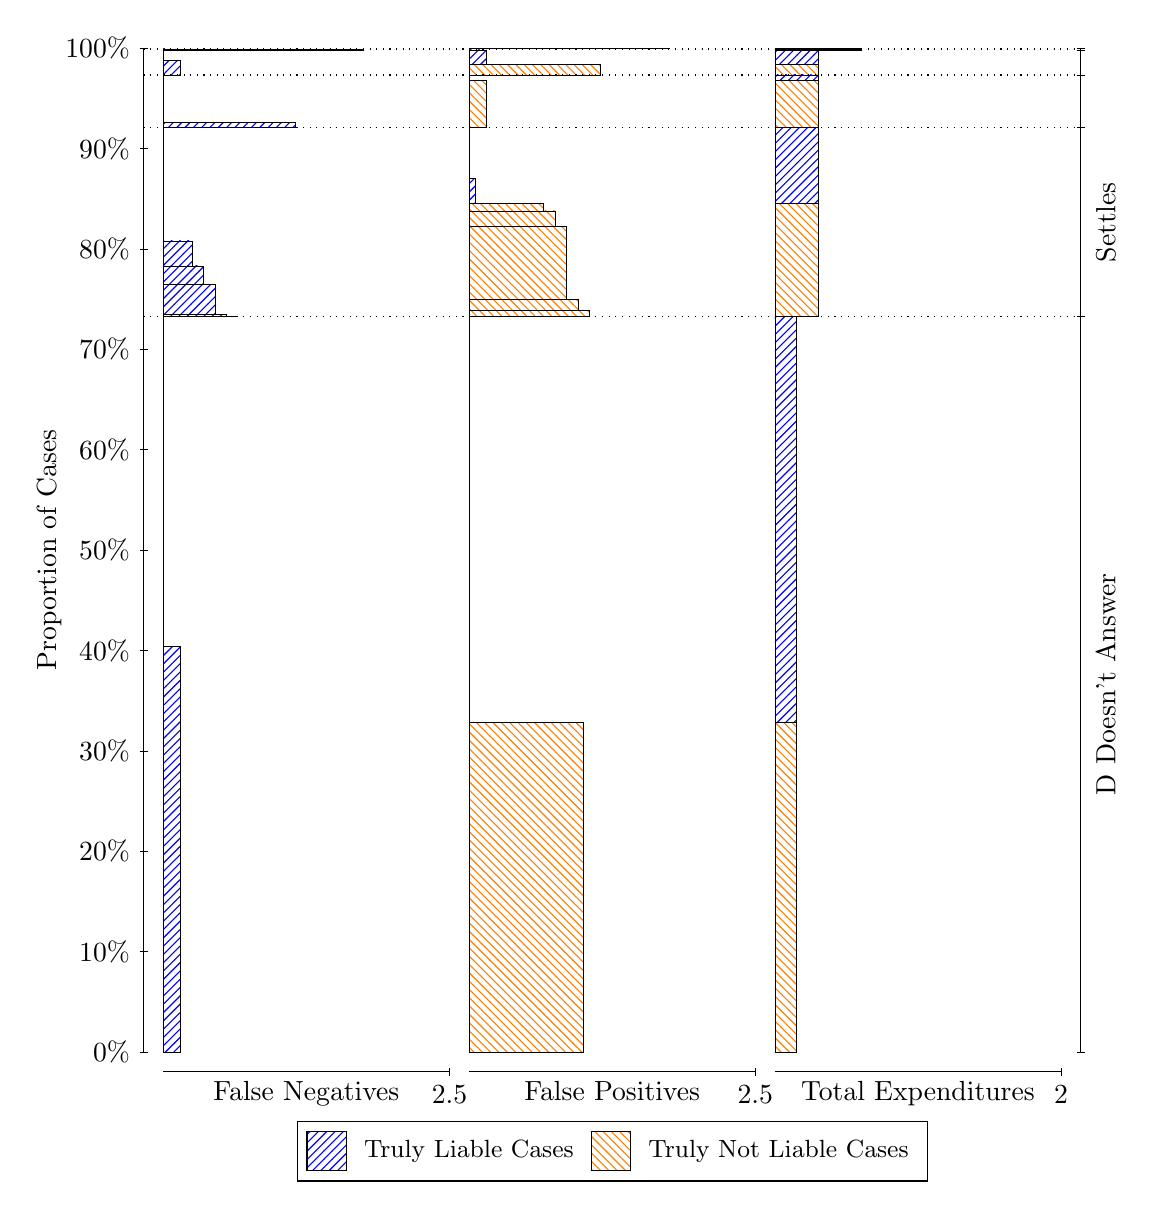
\begin{tikzpicture}
\draw[black, very thin] (1.5,1.75) -- (1.5,14.5);
\node[rotate=90, text=black, anchor=center] at (0.3, 8.125) {Proportion of Cases};
\draw[black, very thin] (1.45,1.75) -- (1.55,1.75);
\node[text=black, anchor=east] at (1.45, 1.75) {0\%};
\draw[black, very thin] (1.45,3.025) -- (1.55,3.025);
\node[text=black, anchor=east] at (1.45, 3.025) {10\%};
\draw[black, very thin] (1.45,4.3) -- (1.55,4.3);
\node[text=black, anchor=east] at (1.45, 4.3) {20\%};
\draw[black, very thin] (1.45,5.575) -- (1.55,5.575);
\node[text=black, anchor=east] at (1.45, 5.575) {30\%};
\draw[black, very thin] (1.45,6.85) -- (1.55,6.85);
\node[text=black, anchor=east] at (1.45, 6.85) {40\%};
\draw[black, very thin] (1.45,8.125) -- (1.55,8.125);
\node[text=black, anchor=east] at (1.45, 8.125) {50\%};
\draw[black, very thin] (1.45,9.4) -- (1.55,9.4);
\node[text=black, anchor=east] at (1.45, 9.4) {60\%};
\draw[black, very thin] (1.45,10.675) -- (1.55,10.675);
\node[text=black, anchor=east] at (1.45, 10.675) {70\%};
\draw[black, very thin] (1.45,11.95) -- (1.55,11.95);
\node[text=black, anchor=east] at (1.45, 11.95) {80\%};
\draw[black, very thin] (1.45,13.225) -- (1.55,13.225);
\node[text=black, anchor=east] at (1.45, 13.225) {90\%};
\draw[black, very thin] (1.45,14.5) -- (1.55,14.5);
\node[text=black, anchor=east] at (1.45, 14.5) {100\%};

\draw[black, very thin] (13.4,1.75) -- (13.4,14.5);
\draw[black, very thin] (13.35,1.75) -- (13.45,1.75);
\node[anchor=west] at (13.35, 1.75) {};
\draw[black, very thin] (13.35,11.088) -- (13.45,11.088);
\node[anchor=west] at (13.35, 11.088) {};
\draw[black, very thin] (13.35,13.489) -- (13.45,13.489);
\node[anchor=west] at (13.35, 13.489) {};
\draw[black, very thin] (13.35,14.158) -- (13.45,14.158);
\node[anchor=west] at (13.35, 14.158) {};
\draw[black, very thin] (13.35,14.477) -- (13.45,14.477);
\node[anchor=west] at (13.35, 14.477) {};
\draw[black, very thin] (13.35,14.493) -- (13.45,14.493);
\node[anchor=west] at (13.35, 14.493) {};
\draw[black, very thin] (13.35,14.5) -- (13.45,14.5);
\node[anchor=west] at (13.35, 14.5) {};

\draw[black, very thin, pattern color=blue, pattern=north east lines] (1.75,1.75) rectangle (1.968,6.8993);
\draw[black, very thin, pattern color=orange, pattern=north west lines] (1.75,6.8993) rectangle (1.75,11.088);
\draw[black, very thin, pattern color=blue, pattern=north east lines] (1.75,11.088) rectangle (2.6947,11.096);
\draw[black, very thin, pattern color=blue, pattern=north east lines] (1.75,11.096) rectangle (2.5493,11.122);
\draw[black, very thin, pattern color=blue, pattern=north east lines] (1.75,11.122) rectangle (2.404,11.5);
\draw[black, very thin, pattern color=blue, pattern=north east lines] (1.75,11.5) rectangle (2.2587,11.734);
\draw[black, very thin, pattern color=blue, pattern=north east lines] (1.75,11.734) rectangle (2.1133,12.052);
\draw[black, very thin, pattern color=orange, pattern=north west lines] (1.75,12.052) rectangle (1.75,13.489);
\draw[black, very thin, pattern color=blue, pattern=north east lines] (1.75,13.489) rectangle (3.4213,13.555);
\draw[black, very thin, pattern color=orange, pattern=north west lines] (1.75,13.555) rectangle (1.75,14.158);
\draw[black, very thin, pattern color=blue, pattern=north east lines] (1.75,14.158) rectangle (1.968,14.347);
\draw[black, very thin, pattern color=orange, pattern=north west lines] (1.75,14.347) rectangle (1.75,14.477);
\draw[black, very thin, pattern color=blue, pattern=north east lines] (1.75,14.477) rectangle (4.2933,14.481);
\draw[black, very thin, pattern color=orange, pattern=north west lines] (1.75,14.481) rectangle (1.75,14.493);
\draw[black, very thin, pattern color=orange, pattern=north west lines] (1.75,14.493) rectangle (1.75,14.496);
\draw[black, very thin, pattern color=blue, pattern=north east lines] (1.75,14.496) rectangle (1.75,14.5);
\draw[black, very thin, pattern color=orange, pattern=north west lines] (5.6333,1.75) rectangle (7.0867,5.9387);
\draw[black, very thin, pattern color=blue, pattern=north east lines] (5.6333,5.9387) rectangle (5.6333,11.088);
\draw[black, very thin, pattern color=orange, pattern=north west lines] (5.6333,11.088) rectangle (7.1593,11.166);
\draw[black, very thin, pattern color=orange, pattern=north west lines] (5.6333,11.166) rectangle (7.014,11.304);
\draw[black, very thin, pattern color=orange, pattern=north west lines] (5.6333,11.304) rectangle (6.8687,12.237);
\draw[black, very thin, pattern color=orange, pattern=north west lines] (5.6333,12.237) rectangle (6.7233,12.432);
\draw[black, very thin, pattern color=orange, pattern=north west lines] (5.6333,12.432) rectangle (6.578,12.525);
\draw[black, very thin, pattern color=blue, pattern=north east lines] (5.6333,12.525) rectangle (5.706,12.843);
\draw[black, very thin, pattern color=blue, pattern=north east lines] (5.6333,12.843) rectangle (5.6333,13.489);
\draw[black, very thin, pattern color=orange, pattern=north west lines] (5.6333,13.489) rectangle (5.8513,14.092);
\draw[black, very thin, pattern color=blue, pattern=north east lines] (5.6333,14.092) rectangle (5.6333,14.158);
\draw[black, very thin, pattern color=orange, pattern=north west lines] (5.6333,14.158) rectangle (7.3047,14.288);
\draw[black, very thin, pattern color=blue, pattern=north east lines] (5.6333,14.288) rectangle (5.8513,14.477);
\draw[black, very thin, pattern color=orange, pattern=north west lines] (5.6333,14.477) rectangle (5.6333,14.489);
\draw[black, very thin, pattern color=blue, pattern=north east lines] (5.6333,14.489) rectangle (5.6333,14.493);
\draw[black, very thin, pattern color=orange, pattern=north west lines] (5.6333,14.493) rectangle (8.1767,14.496);
\draw[black, very thin, pattern color=blue, pattern=north east lines] (5.6333,14.496) rectangle (6.7233,14.5);
\draw[black, very thin, pattern color=orange, pattern=north west lines] (9.5167,1.75) rectangle (9.7892,5.9387);
\draw[black, very thin, pattern color=blue, pattern=north east lines] (9.5167,5.9387) rectangle (9.7892,11.088);
\draw[black, very thin, pattern color=orange, pattern=north west lines] (9.5167,11.088) rectangle (10.062,12.525);
\draw[black, very thin, pattern color=blue, pattern=north east lines] (9.5167,12.525) rectangle (10.062,13.489);
\draw[black, very thin, pattern color=orange, pattern=north west lines] (9.5167,13.489) rectangle (10.062,14.092);
\draw[black, very thin, pattern color=blue, pattern=north east lines] (9.5167,14.092) rectangle (10.062,14.158);
\draw[black, very thin, pattern color=orange, pattern=north west lines] (9.5167,14.158) rectangle (10.062,14.288);
\draw[black, very thin, pattern color=blue, pattern=north east lines] (9.5167,14.288) rectangle (10.062,14.477);
\draw[black, very thin, pattern color=orange, pattern=north west lines] (9.5167,14.477) rectangle (10.607,14.489);
\draw[black, very thin, pattern color=blue, pattern=north east lines] (9.5167,14.489) rectangle (10.607,14.493);
\draw[black, very thin, pattern color=orange, pattern=north west lines] (9.5167,14.493) rectangle (10.607,14.496);
\draw[black, very thin, pattern color=blue, pattern=north east lines] (9.5167,14.496) rectangle (10.607,14.5);
\draw[black, dotted] (1.5,11.088) -- (13.4,11.088);
\draw[black, dotted] (1.5,13.489) -- (13.4,13.489);
\draw[black, dotted] (1.5,14.158) -- (13.4,14.158);
\draw[black, dotted] (1.5,14.477) -- (13.4,14.477);
\draw[black, dotted] (1.5,14.493) -- (13.4,14.493);
\draw[black, very thin] (1.75,1.5) -- (5.3833,1.5);
\node[text=black, anchor=north] at (3.5667, 1.5) {False Negatives};
\draw[black, very thin] (5.3833,1.45) -- (5.3833,1.55);
\node[text=black, anchor=north] at (5.3833, 1.45) {2.5};

\draw[black, very thin] (5.6333,1.5) -- (9.2667,1.5);
\node[text=black, anchor=north] at (7.45, 1.5) {False Positives};
\draw[black, very thin] (9.2667,1.45) -- (9.2667,1.55);
\node[text=black, anchor=north] at (9.2667, 1.45) {2.5};

\draw[black, very thin] (9.5167,1.5) -- (13.15,1.5);
\node[text=black, anchor=north] at (11.333, 1.5) {Total Expenditures};
\draw[black, very thin] (13.15,1.45) -- (13.15,1.55);
\node[text=black, anchor=north] at (13.15, 1.45) {2};

\node[text=black, centered, rotate=90] at (13.72, 6.419) {D Doesn't Answer};
\node[text=black, centered, rotate=90] at (13.72, 12.288) {Settles};





\draw (7.449999999999999,1.5) node[draw=none] (baseCoordinate) {};
\begin{scope}[align=center]
        \matrix[scale=0.5, draw=black, below=0.5cm of baseCoordinate, nodes={draw}, column sep=0.1cm]{
            \node[rectangle, draw, minimum width=0.5cm, minimum height=0.5cm, pattern color=blue, pattern=north east lines] {}; &
            \node[draw=none, font=\small, text=black] (B) {Truly Liable Cases}; &
            \node[rectangle, draw, minimum width=0.5cm, minimum height=0.5cm, pattern color=orange, pattern=north west lines] {}; &
            \node[draw=none, font=\small, text=black] (B) {Truly Not Liable Cases}; \\
            };
\end{scope}

\end{tikzpicture}
\end{document}